\documentclass[a4paper,article]{article}

% Шрифты
\usepackage{fontspec}
\usepackage[14pt]{extsizes}
\setmainfont{Times New Roman}

% Языки
% Русский обязательно идёт вторым. Иначе не работают переносы
\usepackage[english, russian]{babel}

% Параметры страницы
\usepackage[left=3cm, top=2cm, right=1.5cm, bottom=2cm]{geometry}
\usepackage[onehalfspacing]{setspace}

% Параметры текста
% По умолчанию LaTeX не делает отступ после \section. Вроде как оно и не надо, но в тексте ВКР пусть лучше будет. В требованиях отступ описан. Этот пакет своим наличием добавляет этот отступ
\usepackage{indentfirst}
% По умолчанию абзацный отстум меньше требуемого. Задаём конкретный
\setlength{\parindent}{1.25cm}

% Ссылки
\usepackage{color}
\definecolor{Black}{RGB}{0,0,0}
% Без colorlinks вокруг ссылок появляются рамки, недопустимые в ВКР
% Если не зачернить ссылки, то в оглавлении и в других местах будут яркие цвета
\usepackage[colorlinks, allcolors=Black]{hyperref}
% Шрифт для URL
\urlstyle{rm}

% Пункты оглавления
\usepackage{titlesec}
\titleformat{\section}
{\centering\normalfont\bfseries}{\thesection. }{0em}{}
\titleformat{\subsection}
{\centering\normalfont\bfseries}{\thesubsection. }{0em}{}
\titleformat{\subsubsection}
{\centering\normalfont\bfseries}{\thesubsubsection. }{0em}{}
% Список использованных источников
\addto\captionsrussian{\def\refname{Список использованных источников}}

% Таблицы
\usepackage{multicol}
\usepackage{xltabular}

% Перечисления
\usepackage{enumitem}

% Картинки
% Вставка картинок правильная
\usepackage{graphicx}
% "Плавающие" картинки
\usepackage{float}
% Обтекание фигур (таблиц, картинок и прочего)
\usepackage{wrapfig}
% Папка для всех картинок файла
\graphicspath{{images/}}
% Точка в конце названий объекта вместо двоеточия. Например, для Рисунков
\usepackage[labelsep=period]{caption}
% Вместо 'Рис. 1' чтобы было 'Рисунок 1'
\makeatletter
\renewcommand{\fnum@figure}{Рисунок \thefigure}
\makeatother

\begin{document}
    \begin{titlepage}
        \begin{center}
            {\bfseries Министерство науки и высшего образования Российской Федерации \\
            Федеральное государственное автономное образовательное учреждение \\
            высшего образования \\
            <<КАЗАНСКИЙ (ПРИВОЛЖСКИЙ) ФЕДЕРАЛЬНЫЙ УНИВЕРСИТЕТ>>}
        \end{center}

        \begin{center}
            ИНСТИТУТ ВЫЧИСЛИТЕЛЬНОЙ МАТЕМАТИКИ И ИНФОРМАЦИОННЫХ ТЕХНОЛОГИЙ
        \end{center}

        \begin{center}
            КАФЕДРА АНАЛИЗА ДАННЫХ И ТЕХНОЛОГИЙ ПРОГРАММИРОВАНИЯ
        \end{center}

        \begin{center}
            Направление: 09.03.03 – Прикладная информатика
        \end{center}

        \vspace{0mm}

        \begin{center}
            ВЫПУСКНАЯ КВАЛИФИКАЦИОННАЯ РАБОТА \\
            {\bfseries СИСТЕМА ЗАПИСИ НА ПРИЁМ В МЕДИЦИНСКОЕ УЧРЕЖДЕНИЕ}
        \end{center}

        \vfill

        \begin{xltabular}{\textwidth} {
                >{\hsize=0.5\hsize} X
                >{\hsize=0.5\hsize} X }
            \bfseries{Работа завершена:} & \\
            Студент 4 курса & \\
            группы 09-951 & \\
            <<\underline{\hspace{1cm}}>>\underline{\hspace{3cm}} 2023г. & \underline{\hspace{3cm}}/Колесников Д.А. \\
            & \\
            \bfseries{Работа допущена к защите:} & \\
            Научный руководитель & \\
            старший преподаватель & \\
            <<\underline{\hspace{1cm}}>>\underline{\hspace{3cm}} 2023г. & \underline{\hspace{3cm}}/Еникеев И.А. \\
            & \\
            \multicolumn{2}{l}{Заведующий кафедрой анализа данных} \\
            и технологий программирования & \\
            <<\underline{\hspace{1cm}}>>\underline{\hspace{3cm}} 2023г. & \underline{\hspace{3cm}}/Бандеров В.В. \\
        \end{xltabular}

        \vspace{0mm}

        \begin{center}
            Казань — 2023
        \end{center}
    \end{titlepage}

    \newpage

    \setcounter{page}{2}

    \tableofcontents

    \newpage

    \section*{Глоссарий}
    \addcontentsline{toc}{section}{Глоссарий}

    \textbf{РКИБ} - ГАУЗ <<Республиканская клиническая инфекционная больница имени Агафонова>>

    \textbf{Нормализация} - Процесс организации данных в базе данных, нацеленный на повышение её гибкости и защищённости

    \newpage

    \section*{Введение}
    \addcontentsline{toc}{section}{Введение}

        Медицинской отрасли не хватает информатизации. Это устоявшаяся сфера, однако она не соответствует современности: никто не хочет стоять в очередях, вручную заполнять документы, потерять выданный рецепт. В 2018 году Правительство РФ создало национальный проект <<Здравоохранение>>, направленный на улучшение медицины. Одна из задач проекта - перенос Минздравом в электронный формат части услуг: выдача рецептов, запись к врачу, подача заявления на полис, хранение медицинских документов \cite{natsproektzdravoohranenie}.

        На деле перевели услуги в электронный формат не везде. В России 30~000 медицинских учреждений и нужно много времени для внедрения системы в каждое из них. При этом нужно учитывать особенности каждого учреждения - то, что подойдёт больнице в Москве, может не подойти поликлинике из маленького города.

        Одно из учреждений так и не перешедших в электронный формат - Республиканская клиническая инфекционная больница имени Агафонова (далее РКИБ). Сейчас в неё активно внедряюся цифровые технологии, например - оплата услуг. Но некоторые элементы остаются прежними, в частности, запись на приём. С ней то нам и предстоит разобраться.

        \textbf{Цель:} Информатизировать запись на приём в РКИБ

        \textbf{Задачи:}

        \begin{enumerate}[nolistsep]
            \item Изучить предметную область
            \item Проанализировать существующие аналоги
            \item Составить техническое задание
            \item Спроектировать части будущей системы
            \item Реализовать спроектированные части системы
        \end{enumerate}

        \textbf{Объект исследования:} Информатизация в системе здравоохранения

        \textbf{Предмет исследования:} Запись на приём в медицинское учреждение

        \textbf{Структура:} В первой части работы анализируется предметная область и определяется необходимый функционал. Во второй главе будущая система проектируется, в третьей - реализуется. Заключительная, четвертая часть - введение готовой системы в эксплуатацию.

        \newpage

    \section{Предметная область}

    \subsection{Основные сведения}

        РКИБ специализируется на помощи с инфекционными патологиями. Сюда приходят лечиться люди с хроническими заболеваниями и те, кто хочет исследоваться на наличие болезней. Другие поликлиники направляют пациентов в РКИБ, потому что здесь предоставляется большое количество услуг: рентген, диагностика и лечение разных болезней, проведение лабораторных исследований, содержание больных в стационаре.

        В этой больнице нет живых очередей. Каждый пациент записывается на какое-то время и принимается только по записи. Нет ситуаций, когда приходят "Только спросить" или когда требуется неотложная помощь. Этим РКИБ отличается от большинства других поликлиник.

        Врачи сами задают время своего приёма. Они составляют расписание на 2 недели вперёд, но оно может и измениться, например, если врач заболел. Расписание передаётся в регистратуру, где пациентов и записывают на приём.

    \subsection{Существующие решения}

    \subsubsection{Текущее решение проблемы}\label{Текущее решение проблемы}

        На момент начала работы в РКИБ нет никакой информатизированной системы записи на приём. На каждого врача и, иногда, услугу заведена отдельная тетрадь. Пример такой тетради приведён на Рисунке~\ref{fig:Тетрадь на УЗИ+ФС}.

        \begin{figure}[h]

            \centering

            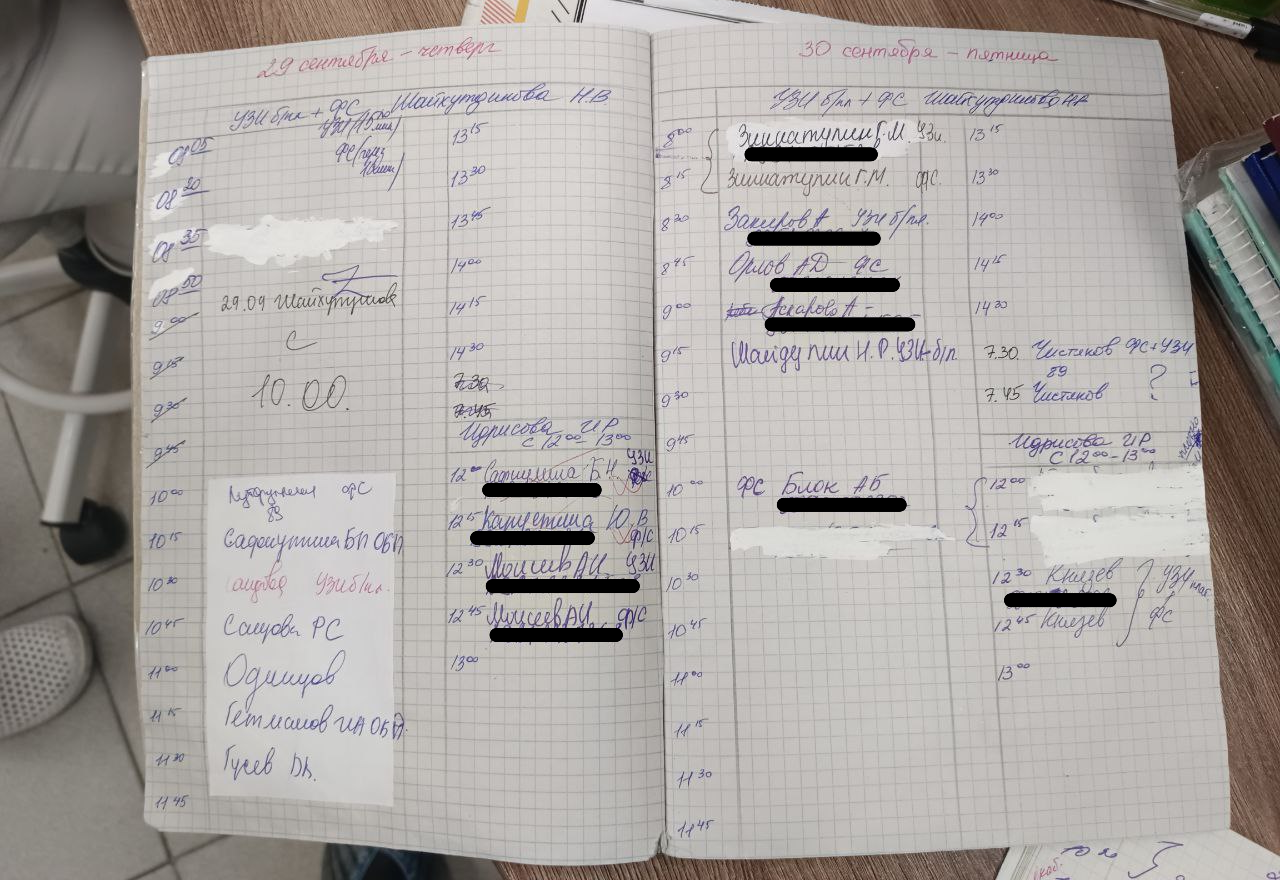
\includegraphics[width=0.8\linewidth]{Пример заполненной тетради на УЗИ+ФС. Чёрным закрашены номера телефонов.png}

            \caption{\centering Пример заполненной тетради на УЗИ+ФС. Чёрным закрашены номера телефонов}

            \label{fig:Тетрадь на УЗИ+ФС}

        \end{figure}

        Пациент, приходя в больницу, иду в регистратуру. Там его вручную записывают в тетрадь на конкретное время к конкретному врачу, вписывают его данные в тетрадь. Далее в указанное время человек приходит к врачу.
        На первый взгляд схема проста и в ней сложно допустить ошибки, но если посмотреть внимательнее, то у неё много недостатков:

        \begin{itemize}[nolistsep]
            \item \textbf{Отсутствие синхронизации.} Если пациент отменил запись, то изменение нужно сделать везде, где было упоминание о приёме.
            \item \textbf{Невозможность копирования.} Каждый врач должен несколько раз в день сверяться с записью к нему, потому что актуальная копия только в регистратуре. При составлении отчётов также требуется переносить сведения о приёме. То есть вручную переписывать сотни строк.
            \item \textbf{Невозможность обработки.} Нужно постараться, чтобы найти данные о пациенте, который приходил месяц назад. Если тетрадь поменялась, то потребуется ещё и находить архивные записи. Восстановить таким образом графики врачей задача тоже не из простых.
            \item \textbf{Дублирование информации.} В РКИБ, по словам сотрудников, много регулярных пациентов. Если кто-то приходит каждый месяц, то в тетрадях он будет записан столько раз, сколько приходил. Редко когда у человека меняется, например, отчество или дата рождения. Эти данные записываются по нескольку раз, хотя это не имеет никакого смысла.
            \item \textbf{Невозможность качественного планирования расписания.} У врачей часто меняется график работы, а в тетради строки фиксированы и ограничены. При любом изменении в графике нужно вручную найти конфликтующие пункты и изменить их.
            \item \textbf{Хранение неактуальной информации.} Человек, поменявший место работы, навсегда в какой-то из тетрадей останется на прошлом.
        \end{itemize}

        Несмотря на недостатки, РКИБ использует этот способ. Всё из-за того, что он прост для понимания, доступен и к нему привыкли. Разработанная в результате система должна быть приближена к этому, чтобы под неё не нужно было долго переучиваться.

    \subsubsection{1С:Медицина}

        <<1С:Медицина>> - решение от компании 1С. Продуманное, сделанное профессионалами, проверенное временем. Пример интерфейса на Рисунке~\ref{fig:Интерфейс 1С:Медицина}. Это мог бы быть хороший вариант, но у него тоже есть недостатки:

        \begin{itemize}[nolistsep]
            \item \textbf{Отсутствие интеграции с существующими системами.} Несмотря на то, что в РКИБ слабо информатизирована, что-то у неё уже есть. Переход на 1С означает отказ от практически всего разработано ранее, либо дополнительные затраты на интеграцию.
            \item \textbf{Избыточность.} Система нацелена на универсальность, поэтому в ней много фунцкций, не нужных этой больнице, их можно было бы упростить. Сложность системы приводит к сложности её внедрения и обслуживания.
            \item \textbf{Цена и поддержка.} Система стоит не малых денег, а поддержка будет требовать дополнительных вложений. При этом, если верить отзывам из открытых источников, поддержка и документация не всегда могут оперативно помочь.
        \end{itemize}

        \begin{figure}[h]

            \centering

            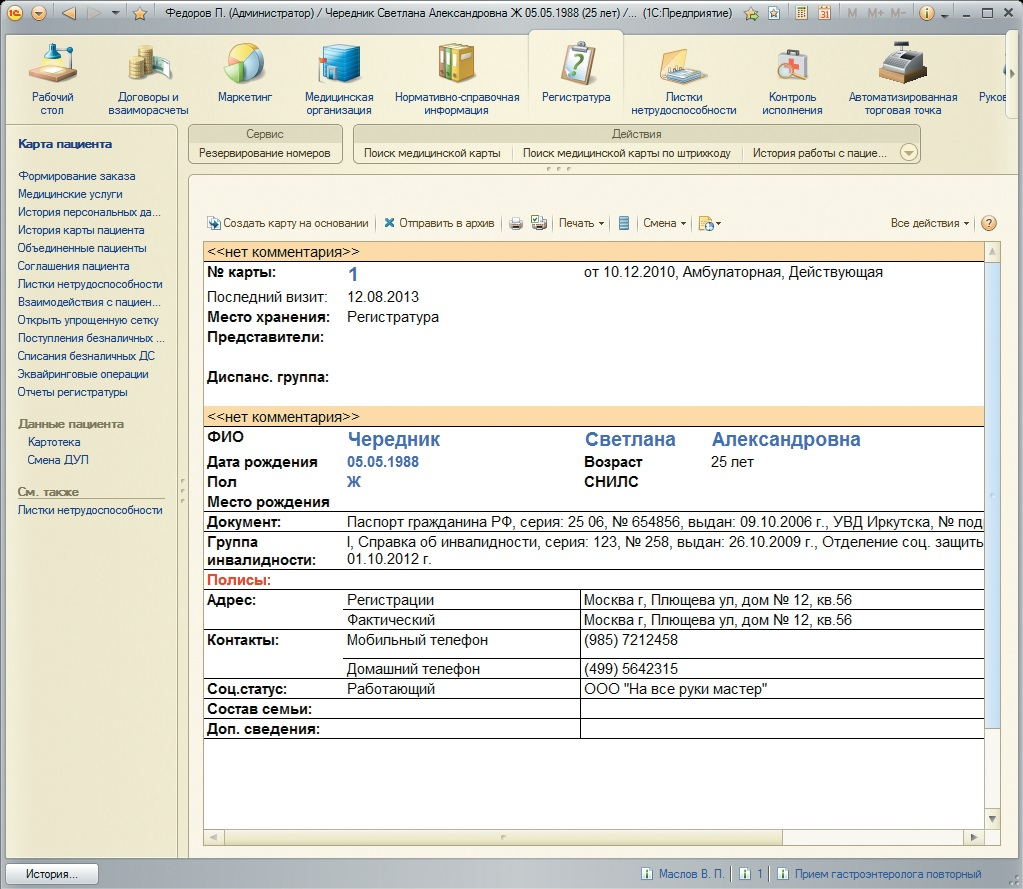
\includegraphics[width=0.6\linewidth]{Интерфейс 1С:Медицина.png}

            \caption{\centering Интерфейс 1С:Медицина}

            \label{fig:Интерфейс 1С:Медицина}

        \end{figure}

    \subsubsection{Другая предлагавшаяся система}

        Разрабатываемая система - не первая, которую хотели внедрить в РКИБ. По словам сотрудников, им уже предлагали готовое решение. Проблема в том, что система не была приспособлена к использованию в этой больнице. Она подходила обычной поликлинике, но РКИБ слишком сильно от них отличается. Здесь нет привычных участков. Обслуживаются не только жители ближайших районов, но и, во том числе, других регионов. Это помешало внедрить её в РКИБ.

        Приспособленность к работе в условиях этой конкретной больницы - важное условие для запуска системы.

    \subsection{Техническое задание}

        В системе выделяются 4 роли:

        \begin{itemize}[nolistsep]
            \item Пациент
            \item Доктор
            \item Регистратор
            \item Администратор
        \end{itemize}

        Каждая из них отличается требуемым функционалом. Диаграмма вариантов использования представленя на Рисунке~\ref{fig:Диаграмма вариантов использования}. Далее рассмотрим их поподробнее.

        \begin{figure}[h]

            \centering

            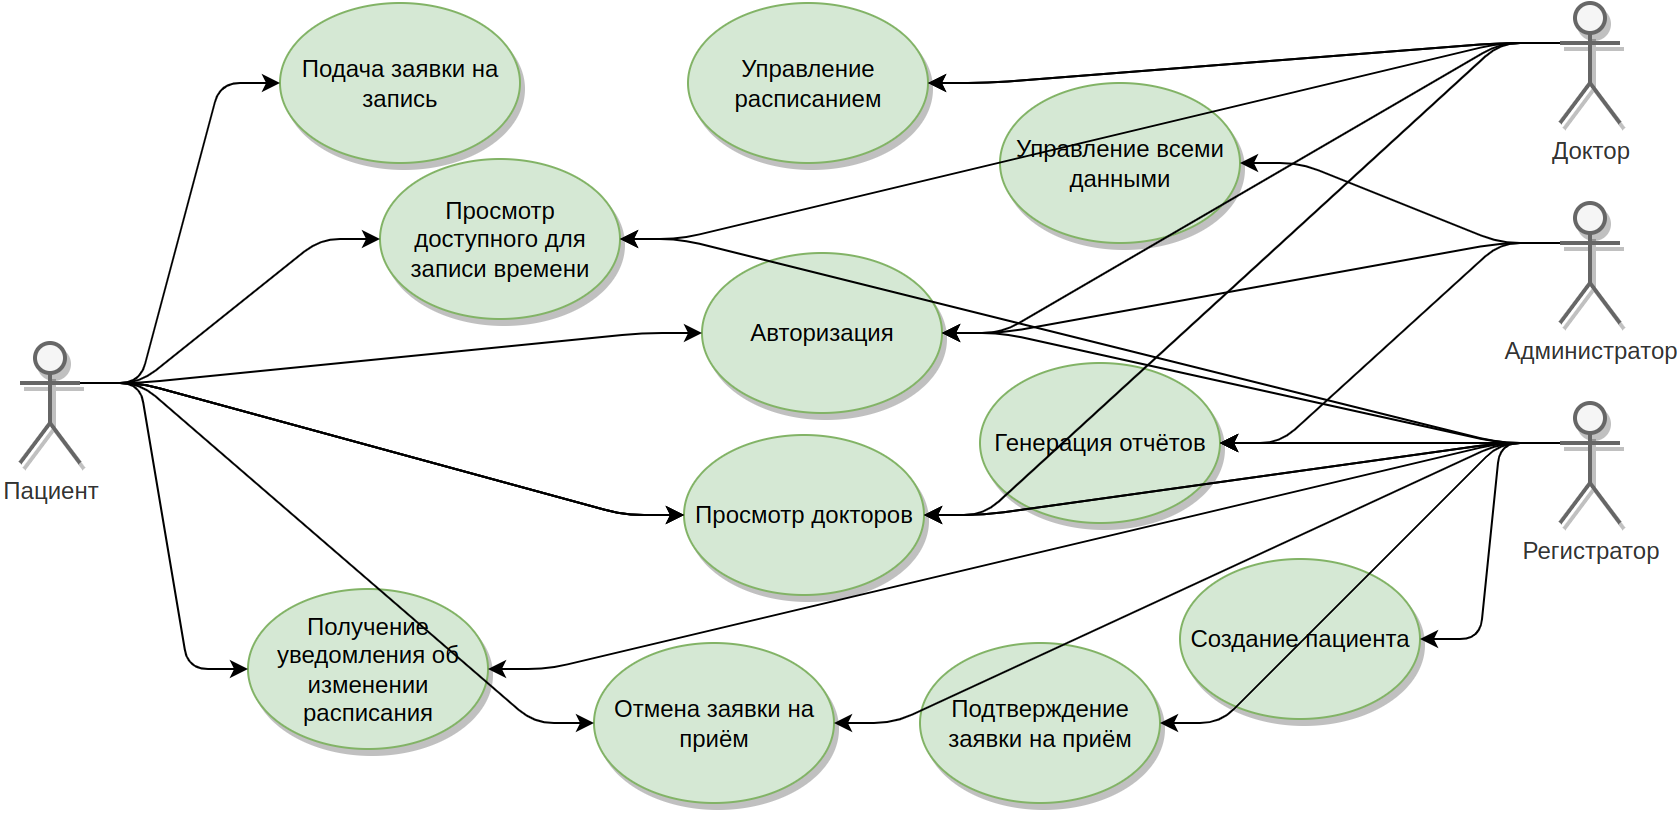
\includegraphics[width=0.8\linewidth]{Диаграмма вариантов использования.png}

            \caption{\centering Диаграмма вариантов использования}

            \label{fig:Диаграмма вариантов использования}

        \end{figure}

    \subsubsection{Пациент}

    \subsubsection{Доктор}

    \subsubsection{Регистратор}

    \subsubsection{Администратор}

    \pagestyle{plain}

    \newpage

    \section{Проектирование}

    \subsection{База данных}

    Для реализации системы потребуется база данных. Её цель - упростить работу с данными для серверной логики.

    \subsubsection{Основные компоненты}\label{Проектирование БД. Основные компоненты}

    Для создания схемы данных нужно проанализировать задачу: Система должна позволять связывать заявки людей на приём и время приёма. Получается, что основных компонентов должно быть 2: \textbf{обращение} и \textbf{расписание}. К этому же можно прийти из пункта~\ref{Текущее решение проблемы}: Для каждого обращения в тетради используется отдельная строка. Для расписания врачей тоже используется одна строка на одно время приёма. Простейшая возможная база данных - простой перенос строк в поля таблиц, получим:

    \begin{itemize}[nolistsep]
        \item \textbf{Обращение:} Содержит данные пациента: ФИО, занятость, адрес для идентификации пациента. Дополнительно содержит направление и диагноз.
        \item \textbf{Расписание:} Включает в себя ФИО врача, услугу, которую он оказывает и данные об обратившемся человеке. Причём приём может быть сразу на 2 ячейки расписания. Связь <<Много к одному>>.
    \end{itemize}

    \subsubsection{Вспомогательные компоненты}\label{Проектирование БД. Вспомогательные компоненты}

    Рассмотрим данные, которые можно было бы вынести в отдельные таблицы, для удобства работы с ними. Дополнительные компоненты можем разделить на 2 категории:

    \begin{itemize}[nolistsep]
        \item Отражающие логику. Они напрямую взяты из тетрадей и понятны обычному человеку.
        \item Упрощающие работу с даными. Нужны только для использования внутри системы.
    \end{itemize}

    Отражающие логику:

    \begin{itemize}[nolistsep]
        \item \textbf{Пациент:} Содержит данные пациент
        \item \textbf{Сотрудник:} Включает в себя
        \item \textbf{Учреждение:} Включает в себя
        \item \textbf{Услуга:} Включает в себя
    \end{itemize}

    Упрощающие работу с данными:

    \begin{itemize}[nolistsep]
        \item \textbf{Человек:} Сущность, объединяющая Пациента и Сотрудника. В обеих таблицах есть ФИО. К тому же аккаунт должен быть и у тех, и у тех. Более того, один и тот же человек может быть и Пациентом, и Сотрудником. Объединение нормализует данные.
        \item \textbf{Статус обращения:} Техническая таблица. Нужна для определения того, что делать с обращением. Например, чтобы отменённое обращение не показывалось в расписании врача.
        \item \textbf{Статус элемента расписания:} Тоже техническая таблица, но для других целей. Например, если врач заболел, то записанные к нему люди будут отдельно обработаны регистратором.
    \end{itemize}

    \subsubsection{Логическая схема данных}

    Исходя из пунктов \ref{Проектирование БД. Основные компоненты} и \ref{Проектирование БД. Вспомогательные компоненты} получаем следующую схему данных:

    \begin{figure}[h]

        \centering

        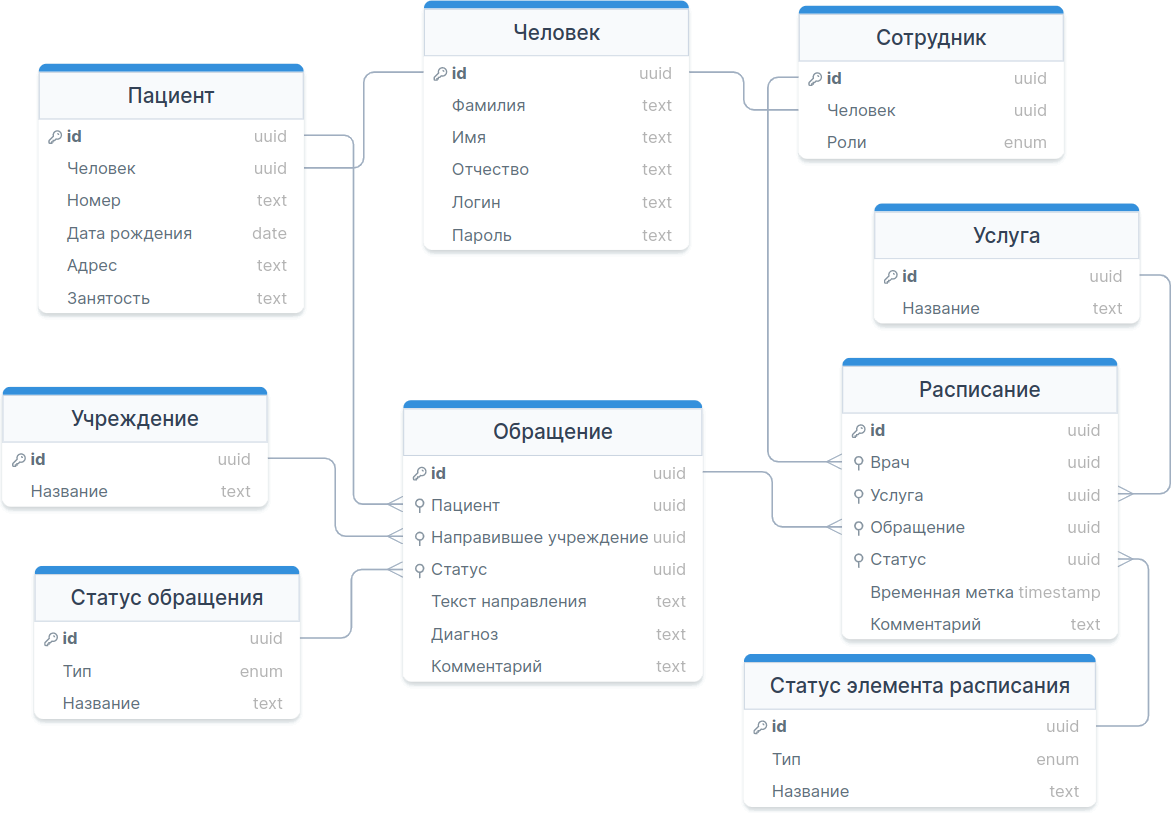
\includegraphics[width=0.9\linewidth]{Логическая схема данных.png}

        \caption{\centering Логическая схема данных}

        \label{fig:Логическая схема данных}

    \end{figure}

    \subsection{Серверная часть}

    \subsection{Клиентская часть}

    \newpage

    \section{Реализация}

    \subsection{Выбор технологий}

    \subsection{База данных}

    \subsection{Серверная часть}

    \subsection{Клиентская часть}

    \newpage

    \section*{Заключение}
    \addcontentsline{toc}{section}{Заключение}

    \newpage

    \addcontentsline{toc}{section}{Список использованных источников}

    \begin{thebibliography}{}
        \bibitem{natsproektzdravoohranenie} Федеральный проект <<Создание единого цифрового контура в здравоохранении на основе единой государственной информационной системы в сфере здравоохранения (ЕГИСЗ)>> - 2019 - 9 августа [Электронный ресурс] - URL: \url{https://minzdrav.gov.ru/poleznye-resursy/natsproektzdravoohranenie/tsifra/} (Дата обращения: 13.12.2022)
    \end{thebibliography}

\end{document}
